\documentclass[letterpaper,12pt]{article}

\usepackage{amsmath}
\usepackage{amssymb,textcomp, esvect,esint}
\usepackage{amsthm}
\usepackage{graphicx,mathtools}
\usepackage{subcaption}
\usepackage[onehalfspacing]{setspace}
\usepackage{subfiles}
\usepackage{framed}

\usepackage{tocvsec2}
%\usepackage[bookmarksdepth=subsection]{hyperref}
\usepackage[hidelinks]{hyperref}
\usepackage{bookmark}
\usepackage[margin=1in]{geometry}
\usepackage{authblk}
\usepackage{titling}
\setlength{\droptitle}{-1in}

\usepackage{mathrsfs,comment}

% place figures and tables where it seems like they should be
\usepackage{float}
\floatplacement{figure}{H}
\floatplacement{table}{H}
\usepackage{color}

\sloppy
\definecolor{lightgray}{gray}{0.5}
\setlength{\parindent}{0pt}

% automatically center figures/tables
\makeatletter
\g@addto@macro\@floatboxreset{\centering}
\makeatother


%%%%%%%%%%%%%%%%%%%%%%%%%%%%%%%%%%%%%%%%%%%%%%%%%%%%%%%%%%%%%%%%%%%%%%
% NEW COMMANDS
\newcommand{\bvec}[1]{\ensuremath{\mathbf{#1}}}

\newtheorem{theorem}{Theorem}
\newtheorem{proposition}{Proposition}
\newtheorem{definition}{Definition}

% section heading formatting
\renewcommand{\thesection}{\arabic{section}.}
\renewcommand{\thesubsection}{\thesection \arabic{subsection}}

\newenvironment{problem}[2][Problem]{\begin{trivlist}
\item[\hskip \labelsep {\bfseries #1}\hskip \labelsep {\bfseries #2.}]}{\end{trivlist}}
    
\newenvironment{solution}[2][Solution]{\begin{trivlist}
\item[\hskip \labelsep {\bfseries #1}\hskip \labelsep {\bfseries #2.}]}{\end{trivlist}}

\newenvironment{code}[2][Code]{\begin{trivlist}
\item[\hskip \labelsep {\bfseries #1}\hskip \labelsep {\bfseries #2.}]}{\end{trivlist}}

\usepackage{sectsty}
\usepackage{titlesec}
\sectionfont{\centering\fontsize{18pt}{1em}\selectfont}
\titlespacing*{\section}
{0pt}{15ex}{12ex}
\titlespacing*{\subsection}
{0pt}{10ex}{8ex}

\title{\fontsize{16pt}{1em}\bfseries Econ 712: Term Project}
\author{Leon Huetsch}


\begin{document}
\maketitle

\subsection*{1 Partial Equilibrium}
\subsubsection*{1.1 Recursive Problem of the Agent}
Bellman equation:
\begin{align*}
v(a,y) &= \max_{(c,a^{\prime})\ge 0} u(c) + \beta \sum_{y^{\prime} \in \mathcal{Y}} \pi \left(y^{\prime} | y \right) v(a^{\prime},y^{\prime}) \\
&\textit{s.t.} \ \ c + a^{\prime} = y + (1+r)a 
\end{align*}
where $\beta = \frac{1}{1+\rho}$ and $y^{\prime}$ follows an AR(1) process given by $\log(y^{\prime}) = \delta \log(y) + \sqrt{1-\delta^2} \varepsilon$ with $\varepsilon \sim N(0,\sigma_Y^2)$. \newline \newline
Plugging in the budget constraint yields the Bellman equation in one variable only.
\begin{align}
v(a,y) &= \max_{a^{\prime}\ge 0} u(y + (1+r)a - a^{\prime}) + \beta \sum_{y^{\prime} \in \mathcal{Y}} \pi \left(y^{\prime} | y \right) v(a^{\prime},y^{\prime})
\end{align}
First order condition withr respect to savings $a^{\prime}$ and the Envelope condition yield
\begin{align*}
u_c (y + (1+r)a - a^{\prime}) &= \beta \sum_{y^{\prime} \in \mathcal{Y}} \pi \left(y^{\prime} | y \right) v_1 (a^{\prime},y^{\prime}) \\
v_1 (a,y) &= u_c (y + (1+r)a - a^{\prime}) (1+r)
\end{align*}
Combining the two equations at the optimal asset holding decision $a^{\prime} (a,y)$ yields the stochastic Euler equation
\begin{equation}
u_c (y + (1+r)a - a^{\prime} (a,y)) = \beta \sum_{y^{\prime} \in \mathcal{Y}} \pi \left(y^{\prime} | y \right) u_c \left( y^{\prime} + (1+r) a^{\prime} (a,y) - a^{\prime} (a^{\prime} (a,y),y^{\prime}) \right) (1+r)
\end{equation}




\subsubsection*{1.2 Infinite Horizon VFI and Simulation}
The files blabla.m and simulationbla.m in the folder Part1\_PE/Functions/ contain the value function iteration and simulation for the infinite horizon case, respectively.



\subsubsection*{1.3 Finite Horizon VFI and Simulation}
The files blabla.m and simulationbla.m in the folder Part1\_PE/Functions/ contain the value function iteration and simulation for the finite horizon case, respectively.




\subsubsection*{1.4 Infinite Horizon Case}
Figures 1 and 2 show the policy function for consumption in the infinite horizon case with low and high variance of the income process, respectively. 
\begin{figure}
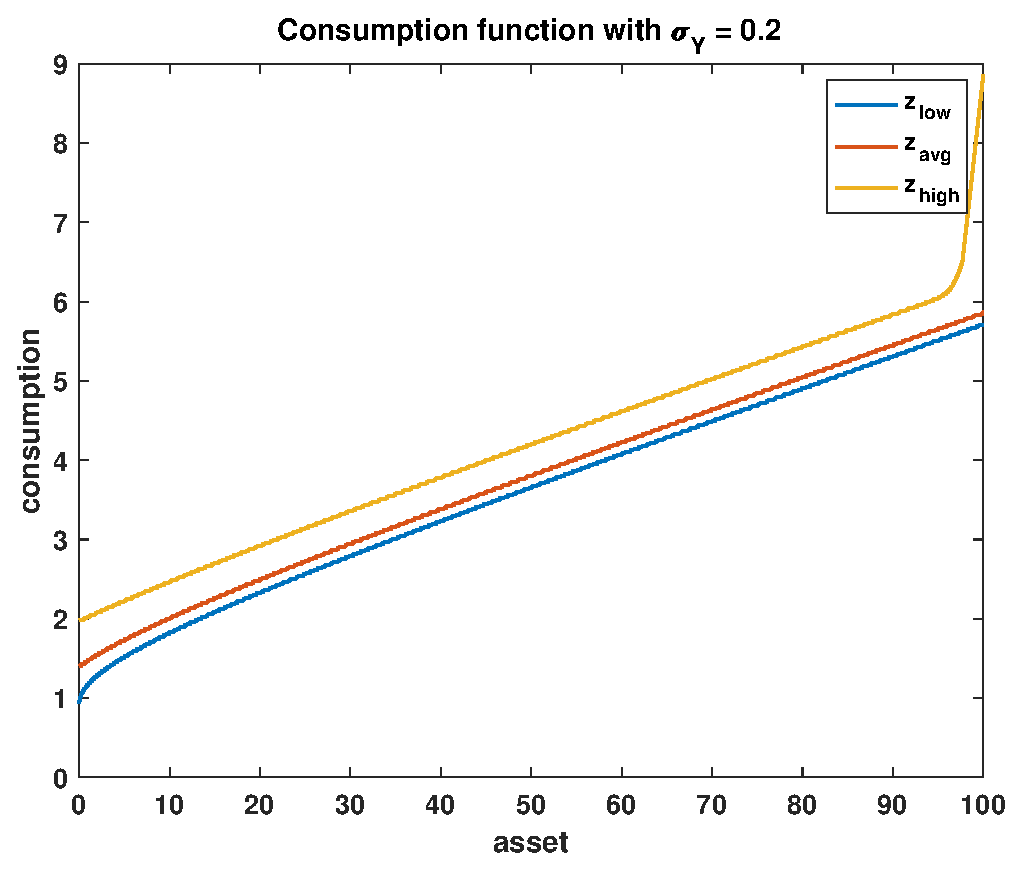
\includegraphics[scale=0.5]{Figures/Part1_PE/consFunc_inf_low}
\caption{Consumption function with low variance $\sigma_Y = 0.2$}
\end{figure}
As expected consumption increases with higher income, shown in the plot by an upward shift of the policy function for higher realizations of $z$. However, the increase in consumption is very low. 
\begin{figure}
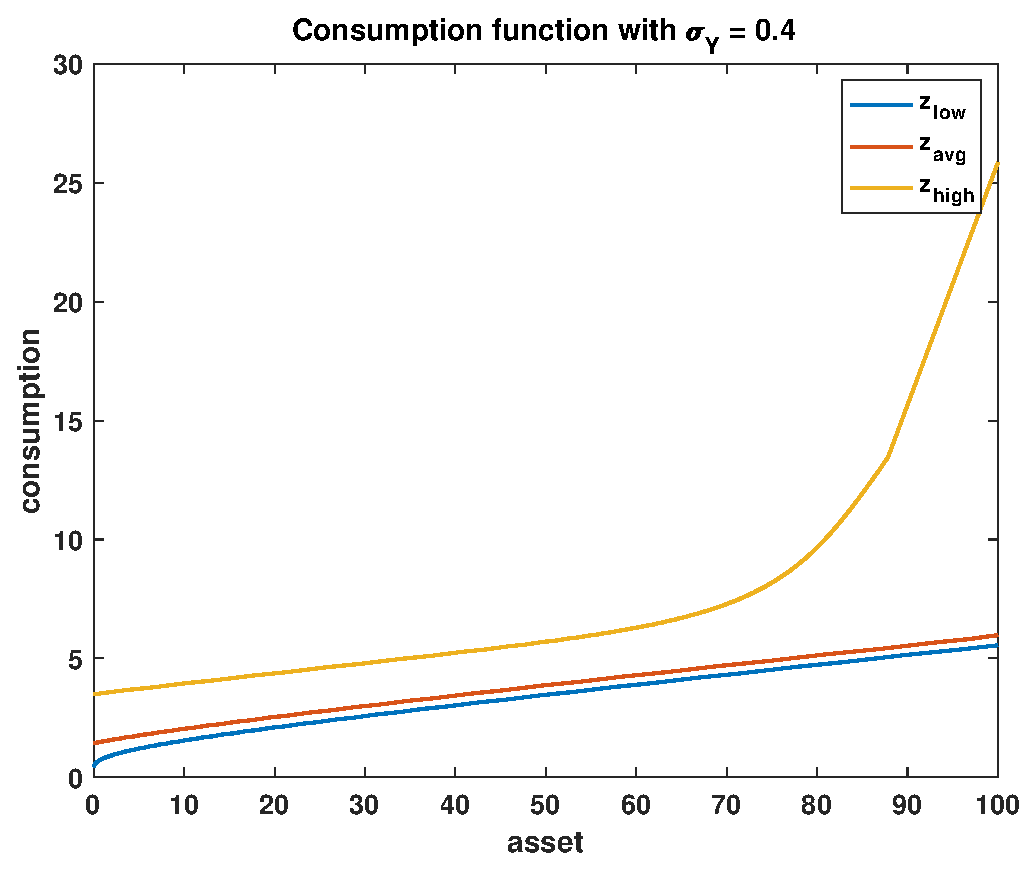
\includegraphics[scale=0.45]{Figures/Part1_PE/consFunc_inf_high}
\caption{Consumption function with high variance $\sigma_Y = 0.4$}
\end{figure}
With high income volatility consumption also increases with more income. However, consumption increases more, meaning 
With low income, $z_{low}$, consumption is higher in the case of lower income volatility.
 The ratio of consumption between the high and low variance case is approximately 3 and constant across asset holdings and realization of the income shock. That is, households increase their consumption by the same factor independent of 
\begin{figure}
\includegraphics[scale=0.5]{Figures/Part1_PE/consFunc_inf_comp1}
\caption{Consumption function with low variance $\sigma_Y = 0.2$}
\end{figure}
\begin{figure}
\includegraphics[scale=0.45]{Figures/Part1_PE/consFunc_inf_comp2}
\caption{Consumption function with high variance $\sigma_Y = 0.4$}
\end{figure}





\subsubsection*{1.5 Finite Horizon Case}
Figures 1 and 2 show the policy function for consumption in the finite horizon case with low and high variance of the income process, respectively. 
\begin{figure}
\includegraphics[scale=0.5]{Figures/Part1_PE/consFunc_fin_low}
\caption{Consumption function with low variance $\sigma_Y = 0.2$ and average income}
\end{figure}
Young households consume less and save more with the same available resources, as they face a longer lifespan and, thus, more future consumption periods which increases their precautionary savings motive.
\begin{figure}
\includegraphics[scale=0.45]{Figures/Part1_PE/consFunc_fin_high}
\caption{Consumption function with high variance $\sigma_Y = 0.4$ and average income}
\end{figure}
The same holds true with high income volatility. The two plots are very similar in levels. However medium income is higher 




\subsubsection*{1.6 Hump in Life Cycle}
Consumption in the previous section is basically flat over the life cycle. The discount rate, $\rho = 0.04$, is larger than the interest rate, $r = 0.02$, thus, agents in principle would like to have a declining consumption profile. However, they are not allowed to borrow as the borrowing constraint is set to $0$. \newline
Relaxing the borrowing constraint yields a declining consumption profile, not a hump, though.
The first difficulty with implementation is to make sure agents cannot choose a Ponzi scheme and never pay back their debt. Since borrowing was permitted, this has not been an issue so far.

\end{document}